	\chapter{Recommendation Systems}

	\begin{bulletedlist}
		\item We are overloaded
		\begin{bulletedlist}
			\item Thousands of news articles and news blogs each day
			\item Millions of movies, books, music tracks online
			\item Several thousands of ad messages sent to us each day
			\item But is it new topic?
		\end{bulletedlist}



		\item From scarcity to abundance
		\begin{bulletedlist}
			\item Historically there was limited resources for products and product advertising:
			\begin{bulletedlist}
				\item Shelf space
				\item Number of hours for TV shows
				\item Number of theaters for Movies
			\end{bulletedlist}
			\item Web enabled near-zero-cost dissimilation of information about products
			\begin{bulletedlist}
				\item Reliance vs Amazon
				\item long tail phenomenon
				\item Cut off point
				\item Area of the curve
			\end{bulletedlist}
		\end{bulletedlist}
		\item Why Recommendation Systems?
		\begin{bulletedlist}
			\item Help user find item of their interest.
			\item Help item provider deliver their items to right user.
			\begin{bulletedlist}
				\item Identify products most relevant to the user
				\item Personalized content
				\item Eg. Top n offers
			\end{bulletedlist}
			\item Help website improve user engagement
		\end{bulletedlist}
		\item Recommender system creates a matching between users and items and exploits the similarity between users/items to make recommendations.
		\item What can be recommended?
		\begin{bulletedlist}
			\item Advertising messages, Movies, Books, Music tracks, News articles, Restaurants, Future friends (Social network sites), Courses in e-learning, Jobs, Research papers, Investment choices, TV programs, Citations, Cloths, Online mates (Dating services), Supermarket goods
		\end{bulletedlist}
		\item User and matching items
		\begin{bulletedlist}
			\item Amazon Users: members, Items: products, books etc. (35\% sales are from recommendation)
			\item Netflix Users: members, Items: movies, TV shows (2/3 rented movies are from recommendation)
			\item LinkedIn Users: members, Items: members
			\item Facebook Users: members, Items: job
			\item Google News (a38\% more click-through are due to recommendation)
		\end{bulletedlist}
	\end{bulletedlist}

	\section{Recommendation Historical Trends}
In 1988, Mr. Joe Simpson, an English mountain climber, wrote a book called \textit{Touching the Void}.  It got good reviews but was considered as modest success and it was soon forgotten.

However, a decade later, an interesting thing happened. Mr. Jon Krakauer wrote a book called \textit{Into Thin Air}, a thriller about a
mountain-climbing tragedy, which became a publishing sensation. Suddenly, \textit{Touching the Void} started to sell again.

Real world examples

	\begin{bulletedlist}
		\item GroupLens(https://grouplens.org/)
		\begin{bulletedlist}
			\item Helped in development of initial recommender systems by pioneering initial collaborative filtering models.
			\item Provided various data sets - MovieLens and BookLens.
		\end{bulletedlist}
		\item Amazon - Did lot of work on implementing commercial recommender systems
		\begin{bulletedlist}
			\item They also implemented lot of computational improvements.
		\end{bulletedlist}
		\item Netflix Prize
		\begin{bulletedlist}
			\item Pioneered Latent Factor/Matrix Factorization models
		\end{bulletedlist}
		\item Google - You Tube
		\begin{bulletedlist}
			\item Hybrid recommendation systems.
			\item Deep Learning Based Systems.
		\end{bulletedlist}
		\item Social Network Recommendations.
	\end{bulletedlist}

Perfect matching item may not exist (see \figurename~\ref{fig:imperfectmatchrecommendationsystem}).

	\begin{figure}[tbh]
		\centering
		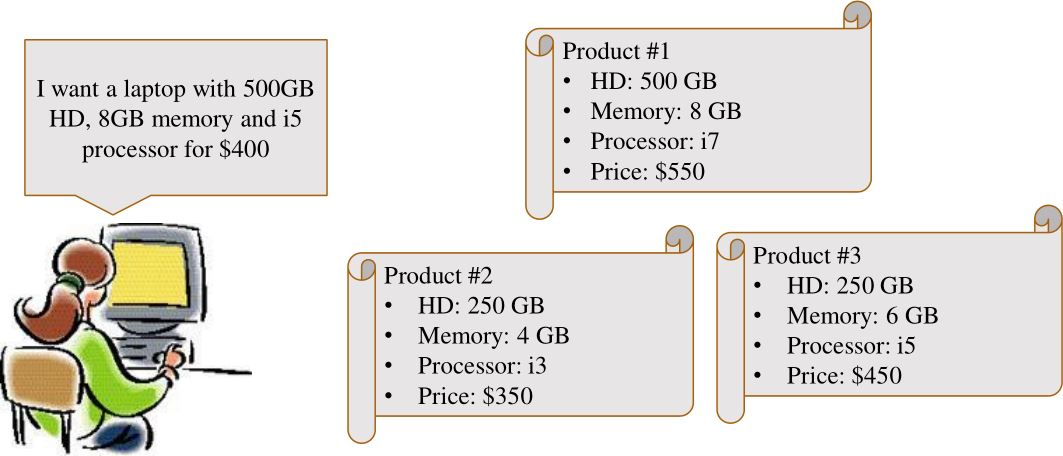
\includegraphics[height=2in]{imperfectmatchrecommendationsystem}
		\caption[Perfect matching recommendation may not exist]{Perfect matching recommendation may not exist.}
		\label{fig:imperfectmatchrecommendationsystem}
	\end{figure}

Types of recommendation systems
	\begin{bulletedlist}
		\item Popularity based recommendations
		\item Classification model based
		\item Content based recommendations
		\item Nearest neighbour collaborative filtering:
		\begin{bulletedlist}
			\item User based
			\item Item based
		\end{bulletedlist}
		\item Hybrid approaches
		\item Association rule mining
	\end{bulletedlist}

Popularity based Recommender System
	\begin{bulletedlist}
		\item Popularity based recommendation system works by recommending items viewed/purchased by most people and rated high.
		\item Recommendations: Ranked list of items by their purchase count / viewed count.
		\item``Popular News''
		\begin{bulletedlist}
			\item Can use context
			\item Purchase history
			\item User and item features
			\item Scalable
		\end{bulletedlist}
		\item Not a personalized recommendation
	\end{bulletedlist}

	\